\documentclass[a4paper,11pt,exos]{nsi} % COMPILE WITH DRAFT

\pagestyle{empty}

\begin{document}
\classe{\premiere spé}
\titre{Corrigé de l'interrogation 1 - A}
\maketitle

\dleft{7.5cm}{
    \exo{}

	On définit sur $\R$ la fonction $f$ par 
	$$f(x)=\dfrac{1}{2}x-3.$$
    Représenter $\courbe{f}$, la courbe représentative de $f$ dans le repère ci-contre.
	}
{

\def\xmin{-5} \def\ymin{-5}\def\xmax{7}\def\ymax{5}
\begin{center}
	\begin{tikzpicture}[scale=.7]
		\reperevl{\xmin}{\ymin}{\xmax}{\ymax}
		\clip (\xmin,\ymin) rectangle (\xmax,\ymax);
        \draw[thick,UGLiRed,domain=\xmin:\xmax,smooth,variable=\x] plot ({\x},{0.5*\x-3});
        \draw (-4,-4) node[UGLiRed,below]{$\mathcal{C}_f$};
	\end{tikzpicture}
\end{center}
}

\exo{}

\dleft{8cm}{
	\def\xmin{-8} \def\ymin{-8}\def\xmax{8}\def\ymax{8}
	\begin{tikzpicture}[scale=.5]
		\reperevl{\xmin}{\ymin}{\xmax}{\ymax}
		\clip (\xmin,\ymin) rectangle (\xmax,\ymax);
		\draw[domain=\xmin:\xmax,smooth,variable=\x] plot ({\x},{-2*\x+6});
		\draw[domain=\xmin:\xmax,smooth,variable=\x] plot ({\x},{3*\x-7});
		\draw[domain=\xmin:\xmax,smooth,variable=\x] plot ({\x},{2/3*\x+1});
		\draw (4,-4) node[below]{$\mathcal{C}_f$};
		\draw (-7,-4) node[below]{$\mathcal{C}_g$};
		\draw (-1,-7) node[below]{$\mathcal{C}_h$};
		
\end{tikzpicture}}
{	On a représenté ici trois fonctions affines $f$, $g$ et $h$.\\
	
	Compléter  sans justifier:\\
	
	$f(x)=\textcolor{UGLiBlue}{-2x+6}$\\
	
	$g(x)=\textcolor{UGLiBlue}{\dfrac{2}{3}x+1}$\\
	
	$h(x)=\textcolor{UGLiBlue}{3x-7}$\\	
	
}

%\newpage
\exo{}
\begin{enumerate}
    \item Donner le tableau de signes des expressions suivantes :
    \begin{multicols}{3}
        \begin{enumalph}
            \item   $3x-2$
            \item 	$(2x+1)(-3x+2)$
            \item	$\dfrac{-5x-2}{x+8}$
        \end{enumalph}
    \end{multicols}

\newpage
    \begin{enumalph}
    \textcolor{UGLiBlue}{
        \item Calcul de la racine :
    \begin{multicols}{2}
        \begin{tabbing}
            $3x-2=0\quad$  \=  $\iff\quad 3x=2$\\
            \>  $\iff\quad x=\dfrac{2}{3}$
        \end{tabbing}       
        \begin{tikzpicture}
            \tkzTabInit[color,lgt=4,espcl=1.5]
            {$x$ /1 ,signe de $ 3x-2$ /1}
            {$-\infty$, $\dfrac{2}{3}$, $+\infty$ }
            \tkzTabLine{, - ,z,+,}
        \end{tikzpicture} 
    \end{multicols}}

    \textcolor{UGLiBlue}{
    \item Calcul des racines :
    \begin{multicols}{2}
        \begin{tabbing}
            $2x+1=0\quad$   \=  $\iff\quad 2x=-1$\\
            \>  $\iff\quad x=-\dfrac{1}{2}$
        \end{tabbing}
        \begin{tabbing}
            $-3x+2=0\quad$   \=  $\iff\quad -3x=-2$\\
            \>  $\iff\quad x=\dfrac{2}{3}$
        \end{tabbing}
    \end{multicols}
    \begin{tikzpicture}
        \tkzTabInit[color,lgt=5,espcl=2]
        {$x$ /1 ,signe de $2x+1$ /1, signe de $-3x+2$ /1, signe de $(2x+1)(-3x+2)$ /1}
        {$-\infty$, $-\dfrac{1}{2}$, $\dfrac{2}{3}$, $+\infty$ }
        \tkzTabLine{, - ,z,+,t,+,}
        \tkzTabLine{,+,t,+,z,-,}
        \tkzTabLine{,-,z,+,z,-,}
    \end{tikzpicture}} 

    \textcolor{UGLiBlue}{
    \item Calcul des racines :
    \begin{multicols}{2}
        \begin{tabbing}
            $-5x-2=0\quad$   \=  $\iff\quad -5x=2$\\
            \>  $\iff\quad x=-\dfrac{2}{5}$
        \end{tabbing}
        \begin{tabbing}
            $x+8=0\quad$   \=  $\iff\quad x=-8$
        \end{tabbing}
    \end{multicols}
    \begin{tikzpicture}
        \tkzTabInit[color,lgt=5,espcl=2]
        {$x$ /1 ,signe de $-5x-2$ /1, signe de $x+8$ /1, signe de $\dfrac{-5x-2}{x+8}$ /1}
        {$-\infty$, $-8$, $-\dfrac{2}{5}$, $+\infty$ }
        \tkzTabLine{, + ,t,+,z,-,}
        \tkzTabLine{,-,z,+,t,+,}
        \tkzTabLine{,-,d,+,z,-,}
    \end{tikzpicture}} 
    \end{enumalph}
    
    \item En déduire les solutions des inéquations suivantes :
    \begin{multicols}{3}
        \begin{enumalph}
            \item   $3x-2\leqslant 0$
            \item 	$(2x+1)(-3x+2)<0$
            \item	$\dfrac{-5x-2}{x+8}\geqslant 0$
        \end{enumalph}
    \end{multicols}
\vspace*{-1cm}
    %\begin{multicols}{3}
    \textcolor{UGLiBlue}{
        \begin{enumalph}
            \item $\mathcal{S}_a=\oif{-\infty}{\dfrac{2}{3}}$
            \item $\mathcal{S}_b=\oio{-\infty}{-\dfrac{1}{2}}\cup\oio{\dfrac{2}{3}}{+\infty}$
            \item $\mathcal{S}_c=\oif{-8}{-\dfrac{2}{5}}$
        \end{enumalph}}
    %\end{multicols}
    
\end{enumerate}


\classe{\premiere spé}
\titre{Corrigé de l'interrogation 1 - B}
\maketitle

\setcounter{section}{0}


\dleft{7.5cm}{
    \exo{}

	On définit sur $\R$ la fonction $f$ par 
	$$f(x)=-\dfrac{1}{2}x+3.$$
    Représenter $\courbe{f}$, la courbe représentative de $f$ dans le repère ci-contre.
	}
{

\def\xmin{-5} \def\ymin{-5}\def\xmax{7}\def\ymax{5}
\begin{center}
	\begin{tikzpicture}[scale=.7]
		\reperevl{\xmin}{\ymin}{\xmax}{\ymax}
		\clip (\xmin,\ymin) rectangle (\xmax,\ymax);
        \draw[thick,UGLiRed,domain=\xmin:\xmax,smooth,variable=\x] plot ({\x},{-0.5*\x+3});
        \draw (-4,4) node[UGLiRed,above]{$\mathcal{C}_f$};
	\end{tikzpicture}
\end{center}
}

\exo{}

\dleft{8cm}{
	\def\xmin{-8} \def\ymin{-8}\def\xmax{8}\def\ymax{8}
	\begin{tikzpicture}[scale=.5]
		\repereal{\xmin}{\ymin}{\xmax}{\ymax}
		\clip (\xmin,\ymin) rectangle (\xmax,\ymax);
		\draw[domain=\xmin:\xmax,smooth,variable=\x] plot ({\x},{3*\x-4});
		\draw[domain=\xmin:\xmax,smooth,variable=\x] plot ({\x},{-2*\x+5});
		\draw[domain=\xmin:\xmax,smooth,variable=\x] plot ({\x},{3/2*\x+2});
		\draw (-2.2,-6) node[below right]{$\mathcal{C}_f$};
		\draw (7,-6) node[below]{$\mathcal{C}_g$};
		\draw (-6,-6) node[below left]{$\mathcal{C}_h$};
		
\end{tikzpicture}}
{	On a représenté ici trois fonctions affines $f$, $g$ et $h$.\\
	
	Compléter  sans justifier:\\
	
	$f(x)=\textcolor{UGLiBlue}{3x-4}$\\
	
	$g(x)=\textcolor{UGLiBlue}{-2x+5}$\\
	
	$h(x)=\textcolor{UGLiBlue}{\dfrac{3}{2}x+2}$\\	
	
}

%\newpage
\exo{}
\begin{enumerate}
    \item Donner le tableau de signes des expressions suivantes :
    \begin{multicols}{3}
        \begin{enumalph}
            \item   $2x-5$
            \item 	$(2x-1)(-5x-3)$
            \item	$\dfrac{-4x+1}{x+3}$
        \end{enumalph}
    \end{multicols}
    
    \newpage
    \begin{enumalph}
    \textcolor{UGLiBlue}{
        \item Calcul de la racine :
    \begin{multicols}{2}
        \begin{tabbing}
            $2x-5=0\quad$  \=  $\iff\quad 2x=5$\\
            \>  $\iff\quad x=\dfrac{5}{2}$
        \end{tabbing}       
        \begin{tikzpicture}
            \tkzTabInit[color,lgt=4,espcl=1.5]
            {$x$ /1 ,signe de $ 2x-5$ /1}
            {$-\infty$, $\dfrac{5}{2}$, $+\infty$ }
            \tkzTabLine{, - ,z,+,}
        \end{tikzpicture} 
    \end{multicols}}

    \textcolor{UGLiBlue}{
    \item Calcul des racines :
    \begin{multicols}{2}
        \begin{tabbing}
            $2x-1=0\quad$   \=  $\iff\quad 2x=1$\\
            \>  $\iff\quad x=\dfrac{1}{2}$
        \end{tabbing}
        \begin{tabbing}
            $-5x-3=0\quad$   \=  $\iff\quad -5x=3$\\
            \>  $\iff\quad x=-\dfrac{3}{5}$
        \end{tabbing}
    \end{multicols}
    \begin{tikzpicture}
        \tkzTabInit[color,lgt=5,espcl=2]
        {$x$ /1 ,signe de $2x-1$ /1, signe de $-5x-3$ /1, signe de $(2x-1)(-5x-3)$ /1}
        {$-\infty$, $-\dfrac{3}{5}$, $\dfrac{1}{2}$, $+\infty$ }
        \tkzTabLine{, - ,t,-,z,+,}
        \tkzTabLine{,+,z,-,t,-,}
        \tkzTabLine{,-,z,+,z,-,}
    \end{tikzpicture}} 

    \textcolor{UGLiBlue}{
    \item Calcul des racines :
    \begin{multicols}{2}
        \begin{tabbing}
            $-4x+1=0\quad$   \=  $\iff\quad -4x=-1$\\
            \>  $\iff\quad x=\dfrac{1}{4}$
        \end{tabbing}
        \begin{tabbing}
            $x+3=0\quad$   \=  $\iff\quad x=-3$
        \end{tabbing}
    \end{multicols}
    \begin{tikzpicture}
        \tkzTabInit[color,lgt=5,espcl=2]
        {$x$ /1 ,signe de $-4x+1$ /1, signe de $x+3$ /1, signe de $\dfrac{-4x+1}{x+3}$ /1}
        {$-\infty$, $-3$, $\dfrac{1}{4}$, $+\infty$ }
        \tkzTabLine{, + ,t,+,z,-,}
        \tkzTabLine{,-,z,+,t,+,}
        \tkzTabLine{,-,d,+,z,-,}
    \end{tikzpicture}} 
    \end{enumalph}



    \item En déduire les solutions des inéquations suivantes :
    \begin{multicols}{3}
        \begin{enumalph}
            \item   $2x-5\geqslant 0$
            \item 	$(2x-1)(-5x-3)>0$
            \item	$\dfrac{-4x+1}{x+3}\leqslant 0$
        \end{enumalph}
    \end{multicols}
    
    \vspace*{-1cm}
    %\begin{multicols}{3}
    \textcolor{UGLiBlue}{
        \begin{enumalph}
            \item $\mathcal{S}_a=\fio{\dfrac{5}{2}}{+\infty}$
            \item $\mathcal{S}_b=\oio{-\dfrac{3}{5}}{\dfrac{1}{2}}$
            \item $\mathcal{S}_c=\oio{-\infty}{-3}\cup\fio{\dfrac{1}{4}}{+\infty}$
        \end{enumalph}}
    %\end{multicols}

\end{enumerate}

\end{document}